% ICEIR 2026 submission draft (Springer LNNS / llncs class).
% Draft status: first full draft, 2026-10-10. Items marked TODO need the authors' input.
% Every number is quoted from the closed result records in docs/ (see docs/paper_outline_iceir2026_20261010.md).
\documentclass[runningheads]{llncs}
\usepackage[T1]{fontenc}
\usepackage{graphicx}
\usepackage{booktabs}
\usepackage{multirow}
\usepackage{amsmath}
\usepackage{url}
\usepackage{pgfplots}
\usepgfplotslibrary{groupplots}
\pgfplotsset{compat=1.17}

\newcommand{\pp}{\,pp}

\begin{document}

\title{Seed and Event Sensitivity in Lightweight SAR Flood Change Detection: A Controlled Negative Result and an Accuracy--Cost Benchmark}
\titlerunning{Seed and Event Sensitivity in Lightweight SAR Flood Change Detection}

% TODO(authors): names, order, affiliations, corresponding author, ORCID.
% TODO(authors): if the submission must be anonymous, keep this block as is.
\author{Author names to be supplied}
\authorrunning{Authors to be supplied}
\institute{Affiliation to be supplied\\
\email{email@to.be.supplied}}

\maketitle

\begin{abstract}
Lightweight change detectors are attractive for mapping floods in synthetic aperture radar
(SAR) imagery, and small-object losses or boundary heads are natural additions when small
urban floods matter. We report what happened when such additions were tested under
pre-specified protocols instead of a single training run. On the UrbanSARFloods dataset we
train a 1.1M-parameter Siamese network in a $2\times 2$ factorial (size-weighted loss,
boundary package) together with two baselines, FC-Siam-Diff and a SAR adaptation of BIT,
over six seeds and two training recipes, and evaluate all 36 runs once on a sealed test set.
Neither component has a consistent effect on validation or test, and every model recovers
only 2--7\% of interior small floods on test. The ranking between model families is stable
across seeds, whereas the ranking among the factorial variants is not. Seed-to-seed variation
concentrates in a single event on each split, but a pre-specified explanation based on flood
fraction is not supported by the test set. A cost study shows that parameter count, counted
FLOPs, GPU latency and CPU latency rank the models in four different orders. We conclude with
reporting recommendations for this task.

\keywords{SAR \and flood mapping \and change detection \and lightweight models \and seed sensitivity \and negative result \and efficiency}
\end{abstract}

\section{Introduction}

Synthetic aperture radar (SAR) observes the ground through cloud and at night, which makes it
the usual data source for mapping floods while they happen~\cite{zhao2024urbansarfloods}.
Public datasets such as Sen1Floods11~\cite{bonafilia2020sen1floods11} have made deep
segmentation models the standard approach for open-area flooding. Urban flooding is harder.
Buildings produce strong and geometry-dependent backscatter, flooded streets are narrow, and
the flooded regions are often only a few pixels wide. The authors of
UrbanSARFloods report that common training choices struggle with this imbalance and that urban
flood detection remains challenging~\cite{zhao2024urbansarfloods}; earlier work found that
interferometric coherence helps in built-up areas~\cite{li2019urbanflood}.

Two further pressures shape model design for this task. First, flood maps are wanted quickly
and, increasingly, close to the sensor, which favours small
models~\cite{mateogarcia2021onboard,codegoni2022tinycd}. Second, the regions that matter most
to responders are small, so it is tempting to add components that target them: losses that
up-weight small connected components~\cite{kofler2022blobloss,rachmadi2024ici} and heads or
losses that sharpen boundaries~\cite{kervadec2019boundary}.

This paper started from exactly that design: a 1.1M-parameter Siamese network with a
size-weighted Tversky loss and a thin boundary head. A single-seed pilot gave results that
could be read as a trade-off between the two components. When we repeated the comparison
under protocols fixed in advance, with new seeds, a second training recipe and finally a
sealed test set, the component effects did not replicate. We therefore report the study as
it is: a controlled negative result, together with what it shows about seed and event
sensitivity and about the cost of the models involved.

We ask three questions. \textbf{RQ1}: do size weighting and a boundary package have a
consistent effect across seeds, two training recipes and a held-out test set? \textbf{RQ2}:
how stable are method rankings against seed and event variation? \textbf{RQ3}: what is the
accuracy--cost trade-off of sub-5M-parameter change detectors on a GPU and on a CPU?

Our contributions are findings rather than a new method:
\begin{itemize}
\item A controlled negative result for both components across six seeds, two recipes and one
sealed test evaluation (Sect.~\ref{sec:components}).
\item An analysis of seed and event sensitivity, including a pre-specified explanation that
the test set did not support (Sects.~\ref{sec:seeds}--\ref{sec:recipe}).
\item An accuracy--cost benchmark of three model families with several cost indicators
measured on two devices (Sect.~\ref{sec:cost}).
\item Protocols, decision rules, code and per-run records that allow each number to be traced.
\end{itemize}

Single-run comparisons are known to be fragile in machine
learning~\cite{reimers2017distributions,bouthillier2021variance,picard2021seed}, and simple
baselines often remain competitive in change detection~\cite{corley2024realitycheck}. The
present study adds a worked case for SAR flood mapping, where validation sets contain only a
handful of events.

\section{Related Work}

\paragraph{SAR flood datasets.} Sen1Floods11 provides georeferenced Sentinel-1 data for 11 flood
events~\cite{bonafilia2020sen1floods11}. Kuro Siwo covers 43 events and provides both ground-range and single-look complex
products~\cite{bountos2024kurosiwo}. UrbanSARFloods contains
8,879 chips of $512\times 512$ pixels from 18 events, with pre- and co-event Sentinel-1
intensity and coherence and separate labels for flooded open areas and flooded urban
areas~\cite{zhao2024urbansarfloods}. We use its intensity channels only.

\paragraph{Bitemporal change detection.} Flood mapping from a pre-event and a co-event image
is a change-detection problem. Fully convolutional Siamese networks~\cite{daudt2018fcsiam}
and transformer-based models such as BIT~\cite{chen2022bit} are common starting points, and
Siamese designs with attention have been applied to SAR flood
pairs~\cite{saleh2024damnet,saleh2024token}. Two recent studies caution that architectural
novelty explains less than it appears to: a plain U-Net remains a top performer on standard
optical benchmarks~\cite{corley2024realitycheck}, and a broad benchmark finds Siamese U-Nets
competitive once efficiency is counted~\cite{tomanic2026benchmark}.

\paragraph{Small regions and boundaries.} The Tversky loss trades false positives against
false negatives~\cite{salehi2017tversky}. Instance-aware losses weight each connected
component rather than each pixel~\cite{kofler2022blobloss,rachmadi2024ici}, and boundary
losses address highly unbalanced segmentation~\cite{kervadec2019boundary}. These ideas were
developed mainly for medical images; small changed regions have also been studied in optical
remote sensing~\cite{cao2020small}. Evaluation guidelines recommend object-level metrics when
objects of very different sizes matter~\cite{maierhein2024metrics}.

\paragraph{Efficiency.} Lightweight change detectors report strong accuracy with few
parameters~\cite{codegoni2022tinycd}, including for SAR flood
mapping~\cite{kacmaz2026lightweight}, and flood segmentation has been developed for use on board small
satellites~\cite{mateogarcia2021onboard}. Dehghani et al.\ show that cost indicators such as
parameters, FLOPs and speed can disagree and argue for reporting several of
them~\cite{dehghani2022efficiency}.

\paragraph{Variance across runs.} Reimers and Gurevych show that the random seed alone can
change conclusions for sequence taggers~\cite{reimers2017distributions}; Bouthillier et al.\
quantify several sources of variance in benchmarks~\cite{bouthillier2021variance}; and
Picard documents seed effects in computer vision~\cite{picard2021seed}.

\paragraph{Gap.} Our literature search was bounded (one search engine, 31 queries on
3~October~2026 and follow-up queries on 10~October~2026) and mostly read at abstract level.
Within those searches we found no SAR flood study that reports recall for small flooded
regions inside a patch, or that reports how method rankings change across training seeds.
This is a statement about our searches, not a claim that no such study exists.

\section{Experimental Design}

\subsection{Data and Splits}

We use the Sentinel-1 intensity channels of UrbanSARFloods~\cite{zhao2024urbansarfloods}:
VH and VV backscatter in decibels for the pre-event and co-event dates. The two flood classes
are merged into one binary flood class. Scenes are cut into non-overlapping
$256\times 256$ patches, and each input channel is standardized with statistics fitted on
training pixels.

Events, not patches, are held out (Table~\ref{tab:data}). The dataset's test events stay as
test; the remaining events are re-partitioned into 12 training and 3 validation events by a
fixed hash rule. \emph{This split differs from the dataset's official partition, so our
numbers are not comparable with those in the dataset paper.} A connected component is
\emph{small} if its area within the patch is at most 35 pixels, the 25th percentile of
training components, and \emph{interior} if it does not touch the patch border or an invalid
pixel.

\begin{table}[t]
\centering
\caption{Event-held-out split. ``Positive'' is the share of valid pixels labelled as flood.
The training positive share was not recorded in our result records.}
\label{tab:data}
\begin{tabular}{lrrrrr}
\toprule
Split & Events & Patches & Positive & Components & Interior small \\
\midrule
Train & 12 & 19,166 & -- & 52,516 & -- \\
Validation & 3 & 4,767 & 1.08\% & 6,745 & 370 \\
Test & 3 & 9,204 & 1.22\% & 27,175 & 4,899 \\
\bottomrule
\end{tabular}
\end{table}

The validation events are Lumberton (2016), Coraki (2022) and Hebei (2023). The test events
are Weihui (2021; 1.03\% positive), Nova Kakhovka (2023; 1.86\%) and Jubba (2023; 0.85\%).
Nova Kakhovka contains 4,379 of the 4,899 interior small components of the test set.

\subsection{Models}

\emph{SmallFlood-CDNet} is a Siamese network with a MobileNetV3-small
encoder~\cite{howard2019mobilenetv3} trained from scratch, a temporal-difference fusion and a
light decoder (1.08M parameters). Its loss is $0.4\,\mathrm{BCE} + 0.4\,\mathrm{Tversky}$ with
false-positive and false-negative weights 0.3 and 0.7~\cite{salehi2017tversky}. We study two
optional components in a $2\times 2$ factorial:
\begin{itemize}
\item \textbf{Size weighting.} Positive pixels of a component with area $a$ receive weight
$1 + \min\bigl(4, (65/a)^{0.5}\bigr)$ in both loss terms, where 65 pixels is the median
training component area.
\item \textbf{Boundary package.} A thin boundary head whose output is added to the change
logits as a residual, with an auxiliary boundary loss of weight 0.2.
\end{itemize}
Variant A uses neither, B size weighting, C the boundary package and D both.

The baselines are \emph{FC-Siam-Diff}~\cite{daudt2018fcsiam} (0.49M parameters) and
\emph{BIT-SAR~v2} (3.49M parameters), our two-channel adaptation of BIT~\cite{chen2022bit}
trained from scratch. Both use $0.5\,\mathrm{BCE} + 0.5\,\mathrm{Tversky}$. The comparison
between families is a whole-method comparison: besides architecture, the baselines differ from
SmallFlood-CDNet in loss coefficients, initialization scheme and training script.

\subsection{Training}

All runs use AdamW with weight decay $10^{-4}$, gradient clipping at 1.0, batch size 8,
15 epochs, 32-bit precision and no data augmentation. Training is fully deterministic: the
same seed reproduces the same weights. Within a seed, variants A--D start from the same
initial weights (apart from the boundary head) and see the same batch order, so differences
between them are paired.

We use two recipes. In the \emph{original} recipe, SmallFlood-CDNet and FC-Siam-Diff use a
learning rate of $3\times 10^{-4}$ and BIT-SAR~v2 uses $10^{-4}$. In recipe \emph{R1} all
models use $10^{-4}$. R1 was selected for variant A in a separate screening study that
compared two learning rates and two schedules on an internal development split of training
events only, without loading the validation events.

\subsection{Metrics}

The primary metric is \emph{event-macro F1}: pixel counts are pooled within each event and
the per-event F1 scores are averaged. We also report pooled pixel F1; component F1 with
one-to-one matching at intersection-over-union $\geq 0.1$; recall of small components,
interior and clipped; boundary F1 with a two-pixel tolerance; and the intersection-over-union
of a two-pixel inner boundary band. The decision threshold is fixed at 0.5. Results are
patch-level; scenes are not reassembled.

The primary checkpoint is the last one (epoch 15). Selecting the best validation epoch chose
transient early peaks in several runs, so best-epoch results are kept only as secondary
information.

\subsection{Staged Protocol and Decision Rules}
\label{sec:protocol}

The study proceeded in stages (Table~\ref{tab:stages}). The discovery stage was exploratory.
From the confirmation stage onward, each stage had a written protocol fixed before any run
of that stage. Stage outcomes were judged by sign-based rules over seeds:
\begin{itemize}
\item \emph{Size weighting does not improve interior-small recall}: supported if
$B-A\le 0$ and $D-C\le 0$ in every seed, contradicted if both are positive in every seed,
otherwise inconsistent.
\item \emph{The boundary package gives no inner-band gain}: the same with $C-A$ and $D-B$.
\item \emph{FC-Siam-Diff is not worse than the heavier models}: supported if FC-Siam-Diff is
at least as good as A and as BIT-SAR~v2 in event-macro F1 in every seed, contradicted if it
is worse than the same comparator in every seed, otherwise inconsistent.
\end{itemize}
No statistical test is applied to pixels, patches or components, because they are not
independent replicates.

\begin{table}[t]
\centering
\caption{Stages of the study. Each stage used seeds with no earlier results.}
\label{tab:stages}
\begin{tabular}{llll}
\toprule
Stage & Recipe & Seeds & Evaluated on \\
\midrule
Discovery & original & 42 & validation \\
Confirmation & original & 1337, 2026 & validation \\
Recipe screening (variant A) & four candidates & 101--103 & internal development split \\
Recipe confirmation & R1 & 201--203 & validation \\
Sealed test, all 36 runs & both & all six & test, once \\
\bottomrule
\end{tabular}
\end{table}

Three disclosures apply. First, the sign rules were written after the discovery seed had
been seen and were applied only to later seeds. For the original-recipe confirmation they
used the best checkpoint for two of the three rules and only the two confirmation seeds; all
later stages use the last checkpoint and three seeds. Second, the test evaluation was
specified in full, including the list of 72 checkpoints (last and best of 36 runs), before
any test array was opened, and it was run once. Third, input normalization statistics were
fitted on all training events, including the two development events used for recipe
screening.

\subsection{Cost Measurement}
\label{sec:costprotocol}

Following Dehghani et al.~\cite{dehghani2022efficiency} we report several indicators for one
pre/post pair of $256\times 256$ patches: parameters; FLOPs counted for convolutions and
matrix multiplications only; serialized weight size; peak GPU memory; batch-1 latency in
PyTorch on an NVIDIA RTX~A6000 at 32-bit and 16-bit precision (100 warm-up and 500 timed
runs, three repetitions); and batch-1 latency in ONNX Runtime on an Intel Xeon Silver~4310
with one and four threads (20 warm-up and 100 timed runs, three repetitions). The server was
shared. GPU repetitions ran only when no other process used the GPU, apart from an idle
process holding 314~MB at 0\% utilization during our measurements. We did not measure an
edge device, and we make no claim about one.

\section{Results}

\subsection{The Two Components Have No Consistent Effect}
\label{sec:components}

Table~\ref{tab:rules} gives the outcome of the three rules on validation and on test for
both recipes. Both component rules are inconsistent in all four settings. On test the
contrasts are small: between $-0.4$ and $+2.3$\pp{} for size weighting and between $-1.1$ and
$+2.2$\pp{} for the boundary package, at an interior-small recall of 2--7\% (Table~\ref{tab:test}).

\begin{table}[t]
\centering
\caption{Rule outcomes and the range of per-seed contrasts in percentage points.
Size: interior-small recall, $B-A$ and $D-C$. Boundary: inner-band IoU, $C-A$ and $D-B$.
Baseline: event-macro F1, FC-Siam-Diff minus A and minus BIT-SAR~v2. Validation with the
original recipe uses two confirmation seeds (Sect.~\ref{sec:protocol}).}
\label{tab:rules}
\footnotesize\setlength{\tabcolsep}{3pt}
\resizebox{\textwidth}{!}{%
\begin{tabular}{llll}
\toprule
Setting & Size weighting & Boundary package & FC not worse (vs.\ A; vs.\ BIT) \\
\midrule
Validation, original & inconsistent & inconsistent & inconsistent \\
 & $[-10.0, +7.0]$ & $[-3.2, +2.1]$ & $[+2.7, +5.5]$; $[-5.6, +2.8]$ \\
Validation, R1 & inconsistent & inconsistent & inconsistent \\
 & $[-1.1, +10.5]$ & $[-0.4, +6.7]$ & $[-3.0, +24.4]$; $[-27.8, +2.0]$ \\
Test, original & inconsistent & inconsistent & contradicted \\
 & $[-0.4, +2.3]$ & $[-1.1, +2.2]$ & $[+6.5, +13.0]$; $[-4.0, -2.2]$ \\
Test, R1 & inconsistent & inconsistent & contradicted \\
 & $[-0.1, +1.8]$ & $[-0.4, +0.9]$ & $[+1.0, +14.1]$; $[-14.3, -3.8]$ \\
\bottomrule
\end{tabular}}
\end{table}

The baseline rule is contradicted on test because BIT-SAR~v2 exceeds FC-Siam-Diff in every
seed of both recipes. FC-Siam-Diff in turn exceeds variant A in all six seeds.

The most direct evidence is in Table~\ref{tab:test}: with 4,899 interior small components in
the test set, every model recalls between 2.4\% and 6.7\% of them on average. Size weighting
does not change this. The small-flood problem that motivated the design is, on this
benchmark, unsolved by all six models.

\begin{table}[t]
\centering
\caption{Test results at the last checkpoint: mean over three seeds, with the range
(max\,$-$\,min) in brackets, in percent. ``Int.\ small'' is interior-small recall.}
\label{tab:test}
\footnotesize\setlength{\tabcolsep}{3pt}
\begin{tabular}{llrrrrr}
\toprule
Recipe & Model & Event F1 & Pixel F1 & Comp.\ F1 & Int.\ small & Bound.\ F1 \\
\midrule
\multirow{6}{*}{Original}
 & A   & 62.0 (4.1)  & 49.9 (7.8)  & 19.3 (1.9) & 3.0 (1.0) & 40.1 (2.3) \\
 & B   & 55.3 (10.3) & 46.3 (6.3)  & 19.1 (1.0) & 3.2 (1.1) & 37.4 (1.2) \\
 & C   & 62.2 (10.0) & 55.6 (13.9) & 18.9 (4.8) & 2.7 (1.8) & 40.0 (9.8) \\
 & D   & 61.3 (10.5) & 52.8 (13.6) & 19.2 (1.9) & 3.4 (1.6) & 39.2 (6.7) \\
 & FC-Siam-Diff & 71.0 (4.5) & 61.1 (15.3) & 19.2 (4.1) & 6.7 (0.7) & 50.2 (5.8) \\
 & BIT-SAR v2   & 73.9 (4.1) & 70.0 (4.2)  & 27.1 (4.9) & 5.1 (2.9) & 52.1 (6.0) \\
\midrule
\multirow{6}{*}{R1}
 & A   & 60.0 (8.6)  & 45.6 (6.0)  & 17.9 (2.7) & 2.4 (1.1) & 37.9 (7.2) \\
 & B   & 58.3 (6.2)  & 44.1 (6.8)  & 18.9 (0.9) & 3.5 (0.2) & 38.1 (2.3) \\
 & C   & 59.8 (11.9) & 47.7 (11.0) & 18.0 (4.3) & 2.7 (2.8) & 37.6 (10.1) \\
 & D   & 59.4 (4.9)  & 48.1 (3.8)  & 19.1 (1.9) & 3.5 (1.8) & 38.7 (2.9) \\
 & FC-Siam-Diff & 65.5 (6.4) & 59.5 (11.8) & 15.9 (4.4) & 4.7 (4.4) & 44.7 (7.6) \\
 & BIT-SAR v2   & 74.2 (8.5) & 70.5 (9.2)  & 25.6 (10.2) & 4.0 (4.1) & 51.4 (13.6) \\
\bottomrule
\end{tabular}
\end{table}

\subsection{Seed Sensitivity and Rank Stability}
\label{sec:seeds}

Figure~\ref{fig:seeds} shows event-macro F1 for every run. On validation, the spread within
one model and recipe reaches 26.7\pp{} (FC-Siam-Diff under R1: 62.3, 83.4 and 56.7) and
16.0\pp{} for variant C. The size-weighting contrast $B-A$ on interior-small recall, measured
at the best checkpoint, was $-13.2$\pp{} in the discovery seed and $+1.6$ and $+7.0$\pp{} in
the two confirmation seeds: a different sign in the seed that prompted the hypothesis than
in the seeds that tested it.

\begin{figure}[t]
\centering
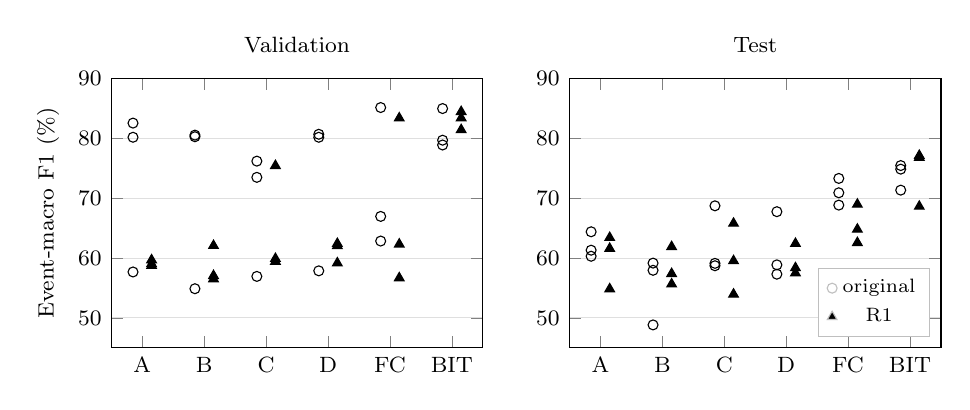
\begin{tikzpicture}
\begin{groupplot}[
  group style={group size=2 by 1, horizontal sep=1.1cm},
  width=6.3cm, height=5.0cm,
  xmin=0.5, xmax=6.5, ymin=45, ymax=90,
  xtick={1,2,3,4,5,6}, xticklabels={A,B,C,D,FC,BIT},
  tick label style={font=\footnotesize}, label style={font=\footnotesize},
  title style={font=\footnotesize}, ymajorgrids, grid style={gray!25},
  ytick={50,60,70,80,90},
  legend style={font=\scriptsize, at={(0.97,0.04)}, anchor=south east, draw=gray!50}]
\nextgroupplot[title={Validation}, ylabel={Event-macro F1 (\%)}]
\addplot[only marks, mark=o, mark size=1.8pt] coordinates {
 (0.85,82.57) (0.85,80.20) (0.85,57.68) (1.85,80.56) (1.85,80.29) (1.85,54.88)
 (2.85,76.21) (2.85,73.50) (2.85,56.94) (3.85,80.20) (3.85,80.70) (3.85,57.87)
 (4.85,85.17) (4.85,66.97) (4.85,62.85) (5.85,85.00) (5.85,78.91) (5.85,79.71)};
\addplot[only marks, mark=triangle*, mark size=2pt] coordinates {
 (1.15,58.74) (1.15,59.03) (1.15,59.68) (2.15,56.51) (2.15,57.06) (2.15,62.08)
 (3.15,75.45) (3.15,59.44) (3.15,59.91) (4.15,59.17) (4.15,62.42) (4.15,62.05)
 (5.15,62.32) (5.15,83.41) (5.15,56.68) (6.15,83.43) (6.15,81.45) (6.15,84.47)};
\nextgroupplot[title={Test}]
\addplot[only marks, mark=o, mark size=1.8pt] coordinates {
 (0.85,60.31) (0.85,64.40) (0.85,61.32) (1.85,59.16) (1.85,57.96) (1.85,48.83)
 (2.85,59.12) (2.85,68.74) (2.85,58.72) (3.85,57.31) (3.85,67.76) (3.85,58.87)
 (4.85,73.32) (4.85,70.92) (4.85,68.86) (5.85,75.47) (5.85,74.87) (5.85,71.36)};
\addplot[only marks, mark=triangle*, mark size=2pt] coordinates {
 (1.15,54.84) (1.15,63.42) (1.15,61.60) (2.15,55.65) (2.15,61.89) (2.15,57.39)
 (3.15,53.95) (3.15,65.80) (3.15,59.54) (4.15,57.51) (4.15,62.43) (4.15,58.36)
 (5.15,68.98) (5.15,64.81) (5.15,62.57) (6.15,77.14) (6.15,68.64) (6.15,76.82)};
\legend{original, R1}
\end{groupplot}
\end{tikzpicture}
\caption{Event-macro F1 of every run at the last checkpoint. Each marker is one seed
(circles: original recipe; triangles: R1). FC: FC-Siam-Diff; BIT: BIT-SAR~v2.}
\label{fig:seeds}
\end{figure}

On test we counted, for each of the 15 pairs of models, whether their order by event-macro F1
is the same in all three seeds of a recipe. Ten pairs are stable under the original recipe
and nine under R1. The pattern is clear. The order \emph{between} families is stable:
BIT-SAR~v2 is above FC-Siam-Diff in all six seeds, and both baselines are above each
SmallFlood-CDNet variant with one exception (variant C exceeds FC-Siam-Diff in one R1 seed,
65.8 against 64.8). The order \emph{among} variants A--D is stable for only one pair under
each recipe. A study that ranked A--D from one seed would have reported an ordering that the
next seed reverses.

\subsection{Variation Concentrates in One Event, but Flood Fraction Does Not Explain It}
\label{sec:events}

On validation, almost all of the seed-to-seed spread comes from one event. Coraki and Hebei
are comparatively stable for every model (F1 of about 90--95\% and 68--86\% under R1), whereas Lumberton F1 ranges from
below 10\% to above 80\%. Under R1, variant A is below 20\% F1 on Lumberton in 42 of its 45
training epochs across the three seeds. The failure is over-prediction: in epochs 11--15 the
SmallFlood-CDNet variants predict 1.5--4.4\% of pixels as flood where the truth is 1.08\%,
while training loss is almost identical across seeds. BIT-SAR~v2 never falls below 20\% on
Lumberton in any of its 90 epochs across the six seeds.

Lumberton has a low flood fraction (about 0.44\% of valid pixels, against 1.08\% for the
validation set as a whole), so we wrote down a rule before opening the test set: the finding \emph{generalizes} if the test event with the
lowest flood fraction has the largest across-seed F1 range in at least 7 of the 12
model-and-recipe groups, and \emph{does not generalize} if in at most 4. The low-fraction
test event is Jubba, and it has the largest range in 4 groups. The outcome is ``does not
generalize''.

Variation on test is still concentrated in one event, but it is Nova Kakhovka, the event with
the \emph{highest} flood fraction and almost all of the small components. It has the largest
range in the other 8 groups. All 14 runs with a test event below 20\% F1 have Nova Kakhovka
as that event, all 14 are SmallFlood-CDNet variants, and in 12 of them the model predicts more
flood pixels than the truth. No FC-Siam-Diff or BIT-SAR~v2 run falls below 20\% on any test
event. We can therefore say that seed sensitivity is event-specific, and that it took the
form of over-prediction on one event per split for the smallest model family. We cannot say
which property of an event causes it; flood fraction is not it.

\subsection{A Recipe Chosen on Held-Out Training Events Did Not Transfer}
\label{sec:recipe}

Because the original recipe collapsed on Lumberton in one of three seeds, we screened four
recipes for variant A on two training events held out as a development split. The lower
learning rate with a constant schedule (R1) gave the highest and most balanced development
score in all three seeds (mean event-macro F1 50.2\% against 37.4\% for the original recipe)
and met a stability rule fixed in advance.

On the real validation events R1 did not help. Variant A reached 58.7, 59.0 and 59.7\%
event-macro F1 in its three R1 seeds, against 82.6, 80.2 and 57.7\% for three other seeds
under the original recipe, with Lumberton F1 of 8.8, 3.8 and 6.1\%. The comparison is not
paired, since the seeds differ, but the direction is plain: the lower learning rate made the
failure consistent instead of removing it. On test the two recipes are close for variant A
(62.0\% and 60.0\%), R1 is worse for FC-Siam-Diff (71.0\% and 65.5\%), and BIT-SAR~v2, which
used the same learning rate in both, is unchanged (73.9\% and 74.2\%).

This stage also exposed a weakness in our own stability rule. It required a small range of
event-macro F1 across seeds and a per-seed F1 on the hardest event of at least half of the
median over seeds. A model that fails in every seed has a low median and passes. Variant A
under R1 was therefore labelled ``stable'' at a Lumberton F1 below 10\%. We noticed this
before the last seed finished, kept the rule as written, and report the label together with
its meaning: consistent, not good. A stability rule needs an absolute floor or a reference
model.

\subsection{Accuracy and Cost}
\label{sec:cost}

\begin{table}[t]
\centering
\caption{Cost for one pair of $256\times 256$ patches. FLOPs count convolutions and matrix
multiplications only. GPU: PyTorch on an RTX~A6000, batch 1, median latency. CPU: ONNX Runtime
on a Xeon Silver~4310, batch 1, median latency. Size and peak memory are for 32-bit weights.}
\label{tab:cost}
\footnotesize\setlength{\tabcolsep}{3pt}
\resizebox{\textwidth}{!}{%
\begin{tabular}{lrrrrrrrr}
\toprule
 & Params & FLOPs & Size & \multicolumn{2}{c}{GPU (ms)} & \multicolumn{2}{c}{CPU (ms)} & Mem. \\
Model & (M) & (G) & (MB) & FP32 & FP16 & 1 thr. & 4 thr. & (MB) \\
\midrule
SmallFlood-CDNet (A, B) & 1.08 & 0.35 & 4.5 & 8.7 & 10.5 & 10.7 & 7.5 & 10.0 \\
\quad + boundary head (C, D) & 1.08 & 0.35 & 4.5 & 9.2 & 10.8 & 10.6 & 8.6 & 10.0 \\
FC-Siam-Diff & 0.49 & 7.02 & 2.0 & 3.0 & 3.8 & 81.4 & 26.0 & 56.0 \\
BIT-SAR v2 & 3.49 & 21.43 & 14.1 & 24.5 & 25.7 & 350.9 & 163.3 & 83.4 \\
\bottomrule
\end{tabular}}
\end{table}

Table~\ref{tab:cost} shows that the four usual indicators rank the models differently.
By parameters, FC-Siam-Diff is the smallest. By counted FLOPs, SmallFlood-CDNet is lightest
by a factor of 20 over FC-Siam-Diff and 62 over BIT-SAR~v2. By GPU latency, FC-Siam-Diff is
fastest and SmallFlood-CDNet is 2.9 times slower despite its low FLOP count. By CPU latency,
SmallFlood-CDNet is fastest: on one thread FC-Siam-Diff is 7.6 times and BIT-SAR~v2 32.8 times
slower. This is the pattern that Dehghani et al.~\cite{dehghani2022efficiency} warn about,
observed here within a single task.

Half precision did not reduce batch-1 latency on this GPU for any model, although it roughly
halved the stored size and reduced peak memory. On the validation split, 16-bit inference
agreed with 32-bit inference on at least 99.989\% of valid pixels and changed no reviewed
metric by more than 0.18\pp{}; ONNX Runtime agreed with PyTorch on all pixels of the 64
patches we compared. Timing on a shared server is noisy, and some repetitions differed
visibly; we report the values as measured.

Figure~\ref{fig:cost} combines Tables~\ref{tab:test} and~\ref{tab:cost}. The model that is
cheapest on a CPU is the least accurate, and the model that is most accurate on test, and the only one that never collapsed on a
validation event, is the most expensive on every indicator. FC-Siam-Diff sits between them,
with the caveat that its accuracy depends more on the recipe.

\begin{figure}[t]
\centering
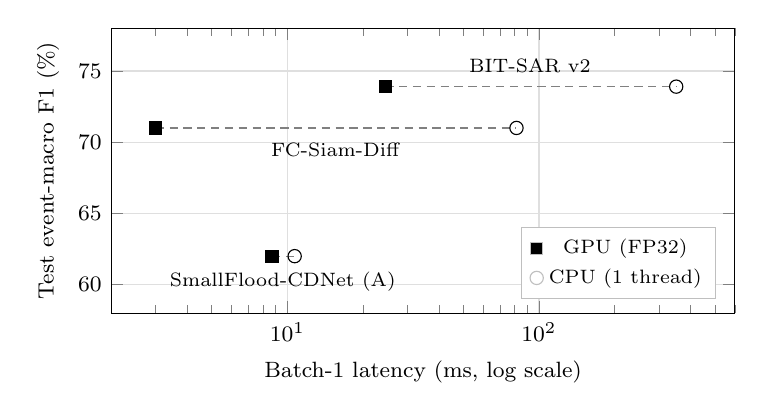
\begin{tikzpicture}
\begin{semilogxaxis}[
  width=9.5cm, height=5.2cm, xmin=2, xmax=600, ymin=58, ymax=78,
  xlabel={Batch-1 latency (ms, log scale)}, ylabel={Test event-macro F1 (\%)},
  tick label style={font=\footnotesize}, label style={font=\footnotesize},
  ymajorgrids, xmajorgrids, grid style={gray!25},
  legend style={font=\scriptsize, at={(0.97,0.05)}, anchor=south east, draw=gray!50}]
\addplot[only marks, mark=square*, mark size=2.2pt] coordinates {(8.7,62.0) (3.0,71.0) (24.5,73.9)};
\addplot[only marks, mark=o, mark size=2.4pt] coordinates {(10.7,62.0) (81.4,71.0) (350.9,73.9)};
\legend{GPU (FP32), CPU (1 thread)}
\draw[densely dashed, gray] (axis cs:8.7,62.0) -- (axis cs:10.7,62.0);
\draw[densely dashed, gray] (axis cs:3.0,71.0) -- (axis cs:81.4,71.0);
\draw[densely dashed, gray] (axis cs:24.5,73.9) -- (axis cs:350.9,73.9);
\node[font=\scriptsize, anchor=north] at (axis cs:9.6,61.6) {SmallFlood-CDNet (A)};
\node[font=\scriptsize, anchor=north] at (axis cs:15.5,70.6) {FC-Siam-Diff};
\node[font=\scriptsize, anchor=south] at (axis cs:92,74.2) {BIT-SAR v2};
\end{semilogxaxis}
\end{tikzpicture}
\caption{Accuracy against latency. Test event-macro F1 is the mean over three seeds under
the original recipe (Table~\ref{tab:test}); latency is from Table~\ref{tab:cost}. Each model
appears twice, once per device, joined by a dashed line.}
\label{fig:cost}
\end{figure}

\section{Discussion}

\paragraph{What the negative result means.} The component effects that looked interpretable
in one seed are within the variation between seeds. The discovery seed suggested that size
weighting \emph{reduced} interior-small recall by 13 points; later seeds showed changes of
either sign, and on a test set with thirteen times more small components the contrasts are
within about two points. We do not conclude that size weighting or boundary supervision can
never help. We conclude that, for this model, dataset and training budget, a benefit could not
be shown, and that a single-seed study would have reported one effect or its opposite
depending on the seed.

\paragraph{What is not established.} We do not know why one event per split triggers
over-prediction in the smallest model family. We tested and rejected one explanation, flood
fraction. We also do not know why BIT-SAR~v2 is robust. It differs from the other models in
architecture, initialization and loss coefficients at once, so its advantage cannot be
attributed to any one of them. Separating these factors is a natural next study.

\paragraph{Recommendations.} For studies of this kind we suggest: (i) report several seeds
with the range, not one run; (ii) report per-event results, because an event-macro score
over three events can be decided by one of them; (iii) report the last checkpoint next to
the best one; (iv) report object-level metrics with their denominators, since pixel F1 hides
a 2--7\% small-region recall; (v) report several cost indicators on more than one device;
and (vi) write the comparison rule down before looking, and say when it was written.

\paragraph{Limitations.} The study uses one dataset, three validation events and three test
events, and three seeds per recipe; the sign rules are conventions, not statistical tests.
Inputs are intensity only, although coherence is known to help in urban
areas~\cite{li2019urbanflood}. Evaluation is patch-level, training lasts 15 epochs without
augmentation, and the split is our own. The recipe was tuned for one variant only. The sign
rules were written after a discovery seed, and one stability rule had the loophole described
in Sect.~\ref{sec:recipe}. Cost was measured on a shared server and not on edge hardware, and
the FLOP counter ignores normalization, activation and attention-softmax operations. Our
literature search was bounded.

\section{Conclusion}

We set out to improve the detection of small urban floods in SAR imagery with a lightweight
model, and instead documented three things. First, neither a size-weighted loss nor a
boundary package had a consistent effect across six seeds, two recipes and a sealed test
set, and all models recovered only a few percent of interior small floods. Second, rankings
between model families were stable while rankings among close variants were not, with the
variation concentrated in one event per split for reasons that flood fraction does not
explain. Third, parameters, FLOPs, GPU latency and CPU latency ordered the models
differently, so ``lightweight'' needs a device and an indicator attached to it.

The open questions are specific: what makes the BIT-based model robust, whether the findings
hold on a second SAR flood dataset, whether coherence changes the picture for urban floods,
and what the models cost on an actual edge device.

% TODO(authors): acknowledgments and funding.
\begin{credits}
\subsubsection{\ackname} To be supplied by the authors. An AI coding assistant was used to
implement and run the experiment scripts and to help draft this manuscript; the authors
reviewed all protocols, results and text and are responsible for the content.
% TODO(authors): confirm or reword the AI-assistance statement according to Springer policy.

\subsubsection{\discintname} The authors have no competing interests to declare that are
relevant to the content of this article.
% TODO(authors): confirm.
\end{credits}

% TODO(authors): data and code availability. UrbanSARFloods is public. Add the repository URL
% here if the submission is not anonymous.

\bibliographystyle{splncs04}
\bibliography{refs}

\end{document}
